
\newpage
\section{Nierzetelne informacje w\,polskiej przestrzeni medialnej}
\subsection{Rodzaje źródeł informacji}
Centrum badania opinii społecznej CBOS przeprowadziło w\,kwietniu 2019 roku badania dotyczące wiarygodności mediów w\,Polsce. Zostały one przeprowadzone metodą wywiadów bezpośrednich na reprezentatywnej próbie losowej dorosłych liczącej 1064 osoby. CBOS przeprowadziło takie badania już po raz drugi, dzięki czemu można porównać jakie zmiany w\,opinii publicznej nastąpiły w\,ciągu dwóch ostatnich lat\cite{CBOSWiarygodnoscMediow2019}.
\par 
Jednym z\,punktów zainteresowań badania była informacja co jest głównym źródłem czerpania informacji o wydarzeniach w\,kraju i\,na świecie Polaków.  Z\,uzyskanych odpowiedzi wynika, że wzrosło znaczenie Internetu używanego w\,takim celu z\,21\% w\,2017 roku do 27\% w\,2019 roku. Jednocześnie zmalała o sześć procent liczba osób deklarująca telewizję jako główne źródło informacji. Inne źródła takie jak radio i\,prasa są najważniejszym źródłem informacji dla relatywnie niewielkiej grupy. Dodatkowo patrząc na zróżnicowanie społeczne od-biorców poszczególnych mediów można zauważyć, że bardzo duże znaczenie ma wiek. W\,grupie młodych dorosłych (osoby w\,wieku 18-24 lata) 60\% deklaruje, że ich głównym źródłem pobierania informacji jest Internet. Patrząc na takie statystyki śmiało można założyć, że znaczenie Internetu w\,dostarczaniu informacji będzie nadal rosło.
\subsubsection{Zaufanie do informacji w\,mediach}
Na zlecenie Komisji Europejskiej międzynarodowy projekt badania opinii publicznej Eurobarometer w\,2018 roku przeprowadził badania na temat fałszywych informacji w\,Internecie\cite{Eurobarometer4642018}. W\,badaniu pytano obywateli wszystkich krajów Unii Europejskiej w\,tym również Polski jakim stopniu ufają różnym typom mediów. Jako zaufanie uznaje się odpowiedź „całkowicie ufam” oraz „raczej ufam” po-daną przez respondenta na pytanie. Polacy mają największe zaufanie do radia 63\% a\,następnie do drukowanej prasy oraz telewizji (odpowiednio 55\% i\,54\%). Patrząc na media publikujące w\,Internecie największym zaufaniem cieszą się portale informacyjne 45\% a\,najmniej respondentów, bo 34\% ma zaufanie do informacji pobieranych poprzez media społecznościowe oraz aplikacje służące do komunikacji. 
\par
Jednak jak wynika z\,poprzednich badań przeprowadzonych przez Eurobarometr prawie jedna piąta użytkowników Internetu w\,Polsce (19\%) pobiera informacje o wiadomościach korzystając z\,mediów społecznościowych. Warto przy tym zwrócić uwagę, że tylko połowa osób kliknie w\,link, aby przeczytać całość artykułu na jego oryginalnej stronie internetowej\cite{Eurobarometer2016}. Takie zachowanie użytkowników umożliwia nierzetelnym stronom na manipulacje informacjami. Zdarza się bowiem, że tytuł przedstawia informację w\,fałszywy sposób a\,dopiero treść artykułu wyjaśnia jak sytuacja naprawdę wygląda. 
\subsection{Fałszywe informacje w\,Internecie}
Badania skupiające się na opinii Polskich internautów o dezinformacji w\,sieci przeprowadził państwowy instytut badawczy NASK na przełomie marca i\,kwietnia 2019\cite{NASKBezpieczneWybory2019}. Zapytano grupy 1000 internautów czy w\,przeciągu 6 ostatnich miesięcy spotkali się w\,Internecie z\,informacjami, które według ich opinii mogły być sfałszowane lub zmanipulowane. Z\,tych badań wynika, że ponad połowa ankietowanych (56\%) spotkała się z\,takim zjawiskiem w\,Internecie w\,przeciągu ostatniego pół roku od chwili zadanego pytania, w\,tym prawie co czwarta osoba zauważa jakąś manipulację informacją codziennie lub kilka razy w\,tygodniu. Tylko 11\% ankietowanych twierdzi, że nie spotkało się z\,zmanipulowanymi informacjami. Pozostałe osoby nie potrafiły odpowiedzieć na to pytanie w\,twierdzący lub zaprzeczający sposób. Część wyników przedstawiono za pomocą diagramu kołowego na rysunku \ref{fig:NASKwyniki}.
\begin{figure}[!h]
	
	\centering 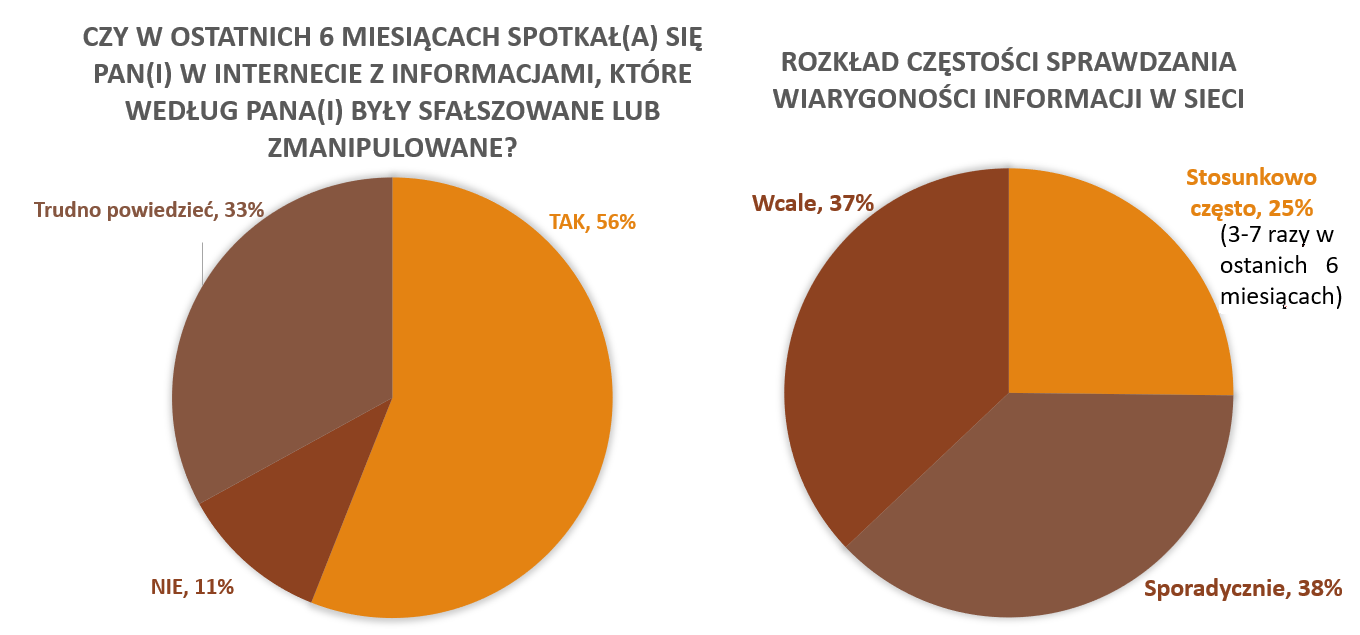
\includegraphics[width=0.9\linewidth]{img/NASKwyniki.PNG}
	\caption{Wybrane wyniki z\,badania opinii Polaków na temat dezinformacji w\,internecie. Opracowanie własne na podstawie źródła: \cite{NASKBezpieczneWybory2019}}
	\label{fig:NASKwyniki}
\end{figure}
\par
\par
Najwięcej respondentów (30\%) jako najczęściej spotykaną przez nich formę dezinformacji i\,manipulacji w\,Internecie określiło fake news, czyli szeroko pojęte fałszywe informacje.  Następnie wskazywano zmanipulowane zdjęcia oraz tzw. trolling czyli celowe prowokowanie do kłótni na forach internetowych poprzez publikowanie nieprawdziwych albo emocjonalnych treści. Jedna piąta ankietowanych nie była jednak w\,stanie powiedzieć jaki typ dezinformacji lub manipulacji najczęściej spotykają.
\par
Tak częste występowanie fałszywych informacji w\,sieci wiąże się z\,tym, że część użytkowników Internetu intencjonalnie lub nieintencjonalnie wchodzi z\,nimi w\,aktywną interakcję przesyłając dalej takie treści lub wyrażając aprobatę poprzez klikanie ‘lubię to’ przy takich publikacjach. Do takiego zachowania w\,czasie ostatniego pół roku przyznało się łącznie prawie 20\% ankietowanych w\,tym 12\% deklaruje, że zrobiło to nie mając świadomości o fałszywości zawartych tam informacji\cite{NASKBezpieczneWybory2019}. 

